\input{head.inc}
  
% Präambelbefehle für die Präsentation
\title[TET: Quasistationäre Felder IV- Induktion]{Quasistationäre Felder IV- Induktion}

\begin{document}
% 
% Frontmatter 
% 
%%%%%%%%%%%%%%%%%%%%%%%%%%%%%%%%%%%%%%%%%%%%%%%%%%%%%%%%%%%%%%%%%%%%%%%%%%%%%%%%%%%%%%%%%%%%%%%%%%%%%%%%%%%%%%%%%%%%%%%%%%%%% 

%% inserts the title page and the table of contents
\maketitle

% 
% Content 
% 
%%%%%%%%%%%%%%%%%%%%%%%%%%%%%%%%%%%%%%%%%%%%%%%%%%%%%%%%%%%%%%%%%%%%%%%%%%%%%%%%%%%%%%%%%%%%%%%%%%%%%%%%%%%%%%%%%%%%%%%%%%%%% 
\section{Quasistationäre Felder IV- Induktion}

\begin{frame}
  \frametitle{Problemstellung}
  \begin{itemize}[<+->]
  \item Ausgangspunkt sind die Maxwellgleichungen im Rahmen der Magnetoquasistatik (MQS), also $\frac{\partial \tetB[v]}{\partial t}\ne \vec{0}$ und $\frac{\partial \verschiebung[v]}{\partial t} = \vec{0}$
    \begin{equation*}
      \divergenz \tetB[v] = 0  \quad \rotation \magfeld[v] = \elstromdichte[v] \quad 
      \divergenz \verschiebung[v] = \laddichte{V}  \quad \textcolor{red}{\rotation \efeld[v] = -\frac{\partial \tetB[v]}{\partial t}} 
    \end{equation*}
  \item Das \alert{Faradaysche Induktionsgesetz} gilt in der \alert{lokalen und instantanen} Formulierung $\rotation \efeld[v] = -\frac{\partial \tetB[v]}{\partial t}$ \alert{immer und überall}.
  \item \alert{Aber:} Bei der Anwendung auf tatsächliche Problemstellungen, die natürlich \alert{ausgedehnt} sind und häufig \alert{Relativbewegungen} eine Rolle spielen, kommt es schnell zu Interpretationsproblemen und \alert{scheinbaren Paradoxien}.
    \begin{itemize}[<+->]
    \item Induzierte Spannung ist \alert{keine Potentialdifferenz}
    \item Ausgedehnte Anordnung, aber \alert{keine Relativbewegung}:
      $$
      U_{ind} = \text{EMK} = \mathcal{E}=\oint_{C(A)} \efeld[v]\cdot\upd\vec{s} = - \frac{\upd }{\upd t} \iint_{A} \tetB[v] \cdot \upd \vec{A} = -\dot{\Phi} \to \text{problemlos}
      $$
      \item aber allgemein: $\rotation \efeld[v] = -\frac{\partial \tetB[v]}{\partial t} \to \oint_{\textcolor{red}{C(A(t))}} \efeld[v]\cdot\upd\vec{s} = -\iint_{\textcolor{red}{A(t)}} \frac{\partial \tetB[v]}{\partial t} \cdot \upd \vec{A}$
    \end{itemize}
  \end{itemize}
\end{frame}


\begin{frame}
  \frametitle{EMK vs Potentialdifferenz}
  \begin{itemize}[<+->]
  \item Wegen $\rotation \efeld[v] = -\frac{\partial \tetB[v]}{\partial t} \ne \vec{0}$ ist das elektrische Feld \alert{kein Gradientenfeld}
  \item Spannungen im Sinne von \alert{Potentialdifferenzen} sind \alert{nicht definiert}, weil es kein dem E-Feld zugeordnetes Skalarpotential gibt.
    \item $\text{EMK} = U_{ind}=\mathcal{E}$ ist \alert{keine Potentialdifferenz} $\to$ Spannungsmessungen zwischen identischen Punkten sind \alert{nicht wegunabhängig.}
    \end{itemize}\pause
    
  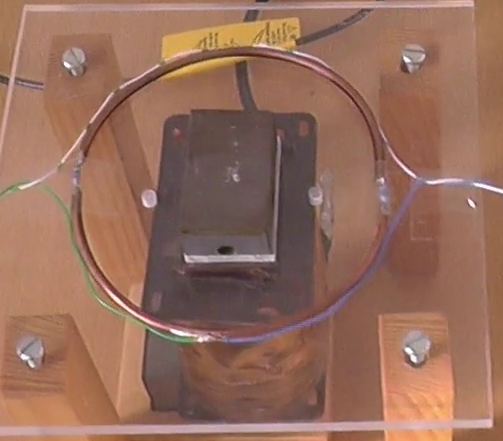
\includegraphics[width=5cm]{ParadoxeSpannungsmessung-teil.png}\hspace*{1cm}\pause
  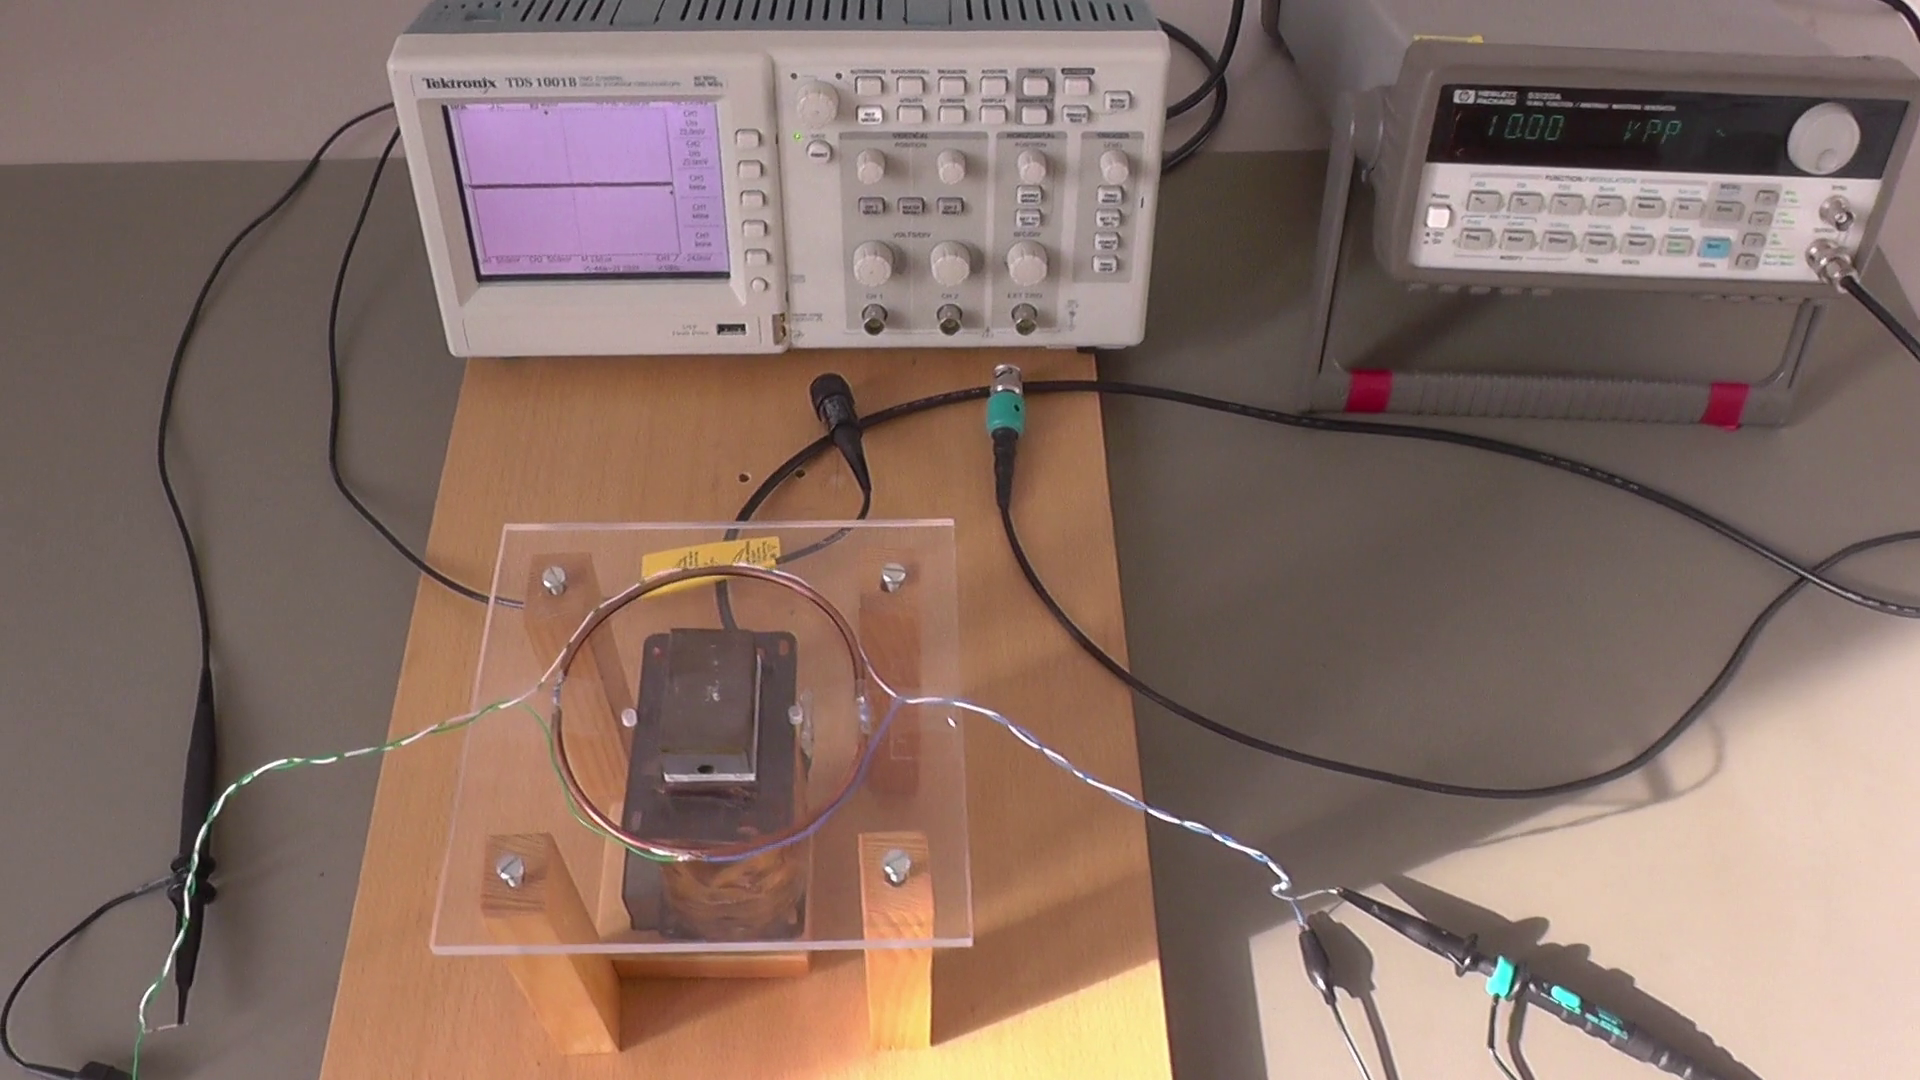
\includegraphics[width=5cm]{ParadoxeSpannungsmessung.png}
\end{frame}

\begin{frame}
  \frametitle{Scheinbar paradoxe Spannungsmessung}
  \begin{itemize}[<+->]
  \item Messung der Spannung zwischen zwei identischen Punkten.
    \only<1|handout:0>{\incfig{paradoxeSpanungsmessung}}
    \only<2->{\incfig{paradoxeSpanungsmessung2}}
  \item
    $$
    \mathcal{E} + I (R_1+R_2)= 0 \quad U_1+\mathcal{E} + I R_2 = 0 \quad -U_2+\mathcal{E} + I R_1 = 0 \to \boxed{\frac{U_1}{U_2} = -\frac{R_1}{R_2}} 
    $$
  \end{itemize}
\end{frame}

\begin{frame}
  \frametitle{Anordnungen mit Relativbewegung}
  \begin{columns}
    \begin{column}{.4\textwidth}
  \resizebox{\columnwidth}{!}{\begin{tikzpicture}[line width = 1.2pt, line join=round,x=1cm,y=1cm,>=stealth, scale = 0.4]
	% Grenzfläche
	\draw [color = darkgreen] (0,-5) -- (0,10);
	% Geschwindigkeit
	\draw [color = blue,->] (3,1) -- ++(2,0) node [anchor = west] {$ \geschw[v] $};
	% Leiterschleife
	\draw (-6,0) rectangle (3,7);
	\filldraw [fill = white, draw = black] (3,3.5) circle (1);
	\draw [->] (1.5,2) -- ++(3,3);
	% Normalenvektor der Fläche
	\coordinate (a) at (-2,3.5);
	\filldraw (a) circle (1.5pt);
	\draw (a) circle (8pt);
	\draw (a) node [anchor = west] {$ \ \flaeche[v] $};
	% Höhe der Schleife
	\draw [|<->|] (-7,0) -- ++(0,7) node [anchor = east, midway] {$ h $};
	% Durchflossene Schleife
	\draw [|<->|] (0,-1) -- ++(-6,0) node [anchor = north, midway] {$ x $};
	\draw (-1,-3) node [anchor = north east] {$ x(t = 0) = x_0 $};
	% Magnetisches Feld
	\coordinate (ma) at (-6,9);
	\coordinate (mb) at (-3,9);
	\coordinate (mc) at (1,9);
	\draw [color = red] (ma) circle (1.5pt);
	\draw [color = red] (ma) circle (8pt);
	\draw [color = red] (ma) node [anchor = east] {$ \tetB[v] = \tetB[v]_0\  $};
	\draw [color = red] (mb) circle (1.5pt);
	\draw [color = red] (mb) circle (8pt);
	\draw [color = red] (mc) node [anchor = west] {$ \tetB[v] = \vec{0} $};
\end{tikzpicture}}
    \end{column}
    \begin{column}{.6\textwidth}
  \begin{itemize}[<+->]
  \item Offenbar gilt $\frac{\partial \tetB[v]}{\partial t} = \vec{0}$:
    $$
    \to \oint_{C(A)} \efeld[v]\cdot\upd\vec{s} = -\iint_{A} \frac{\partial \tetB[v]}{\partial t} \cdot \upd \vec{A} = 0 \text{ \alert{???}}
    $$
  \item Experiment: \alert{es wird eine Spannung induziert}
  \item Erklärungsausweg: \alert{Lorentzkraft} auf Ladungsträger im bewegtem Leiter
  \item zulässig, aber völlig \alert{unbefriedigend} im Rahmen der Feldtheorie
  \item Tatsächlich läßt sich dieses Problem auf zwei Weisen lösen
    \begin{itemize}[<+->]
    \item \alert{Mathematisch} mit der vollständigen \alert{Leibniz-Regel für Integrale}
     \item \alert{Physikalisch} mit der \alert{Speziellen Relativitätstheorie}
      \end{itemize}
  \end{itemize}
      \end{column}
    \end{columns}
\end{frame}

\begin{frame}
  \frametitle{Leibniz Integralregel --- Ableitung unter dem Integral}
  \begin{itemize}[<+->]
  \item Eindimensionaler Fall noch relativ bekannt:
    $$
    \frac{\upd}{\upd t} \left( \int\displaylimits_{a(t)}^{b(t)} f(t,x)\upd x \right) = f(t,b(t)) \frac{\upd }{\upd t}b(t)  - f(t,a(t)) \frac{\upd }{\upd t}a(t) +  \int\displaylimits_{a(t)}^{b(t)} \frac{\partial}{\partial t}f(t,x)\upd x 
    $$
  \item 3D Form (Flanders, \enquote{Differentiation under the Integral Sign}, The American Mathematical Monthly, Vol. 80, No. 6, 615-627, (1973)):
    $$
    \frac{\upd}{\upd t}  \iint_{A(t)} \vec{f} (\ortsvektor[v], t) \cdot \upd\vec{A} = \iint_{A(t)} \left( \frac{\partial}{\partial t}\vec{f}(\ortsvektor[v], t) + \left[ \divergenz\; \vec{f}(\ortsvektor[v], t) \right] \vec{v} \right) \cdot \upd\vec{A} - \oint\displaylimits_{C(A(t))}
    \vec{v} \times  \vec{f}(\ortsvektor[v], t) \cdot \upd\vec{s}   $$
  \item Hier \(\divergenz \tetB[v]=0\):
    $$
    \frac{\upd}{\upd t}  \iint_{A(t)} \tetB[v] (\ortsvektor[v], t) \cdot \upd\vec{A} = \iint_{A(t)} \frac{\partial}{\partial t}\tetB[v](\ortsvektor[v], t) \cdot \upd\vec{A} - \oint\displaylimits_{C(A(t))}
    \vec{v} \times \tetB[v](\ortsvektor[v], t) \cdot \upd\vec{s}   $$
  \item Damit folgt dann:
    $$
   \boxed{\mathcal{E}=\text{EMK}=U_\text{ind} = \oint\displaylimits_{C(A(t))} \left( \efeld[v] + \vec{v} \times \tetB[v]\right) \cdot\upd\vec{s} = - \frac{\upd}{\upd t}  \iint_{A(t)} \tetB[v] \cdot \upd\vec{A}  = -\dot{\Phi}}
    $$
\end{itemize}
\end{frame}


\begin{frame}
  \frametitle{Spezielle Relativitätstheorie}
  \begin{itemize}[<+->]
  \item Axiome der SRT ($\to$ Axiomatische Grundlagen)
      \begin{itemize}[<+->]
      \item \alert{Relativitätsprinzip} - Naturgesetze haben in Inertialsystemen die gleiche Form
        \item \alert{Universalität der Lichtgeschwindigkeit} - Die Lichtgeschwindigkeit im Vakuum ist eine universelle Konstante, die in allen Inertialsystemen den gleichen Wert hat. 
        \end{itemize}
      \item Ladungserhaltung folgt im Rahmen der SRT ($\to$ Noether-Theorem, Noether-Strom)
      \item Bekannt: \alert{Lorentztransformation}, \alert{Raum-Zeit}, \alert{Längenkontraktion}, \alert{Zeitdilatation}
      \item Hierbei tauchen immer folgende Faktoren auf:
        $$
        \beta = \frac{v}{c}, \beta \in [0, 1] \text{ und } \gamma = \sqrt{\frac{1}{1-\beta^2}}, \gamma \in [1,\infty) 
        $$
        \begin{tabular}{c||c|c|c|c|c|c |c|c|c|c}
          $\beta$ & 0 & 0.1 & 0.2 & 0.3 & 0.4 & 0.5 & 0.6  & 0.8  & 1.0\\
          \hline
     $\gamma$ & 1 & 1.005 & 1.021 & 1.048 & 1.091 &  1.155 &  1.25 & 1.667  & $\infty$
        \end{tabular}
        \item Gute Näherung für nicht-relativistische Geschwindigkeiten: \alert{$\gamma = 1$}
\end{itemize}
\end{frame}

\begin{frame}
  \frametitle{Transformation der Felder}
  \begin{itemize}[<+->]
  \item Es sei S' ein Inertialsystem, das sich mit $\vec{v}=\text{const.}$ relativ zum Laborsystem S bewegt
  \item Mit $\vec{v} = v \vu{v}$ können die Felder in S in longitudinale und transversale Anteile zerlegt werden:
    \begin{align*}
      \efeld[v] & = \efeld[v]_\parallel + \efeld[v]_\perp = (\vu{v} \cdot \efeld[v]) \vu{v} + \vu{v} \times (\vu{v} \times \efeld[v]) \\  
      \tetB[v] & = \tetB[v]_\parallel + \tetB[v]_\perp = (\vu{v} \cdot \tetB[v]) \vu{v} + \vu{v} \times (\vu{v} \times \tetB[v])
    \end{align*}
  \item Im System S' ergeben sich diese Felder dann zu:
    \begin{align*}
      \efeld[v]' & = \efeld[v]_\parallel + \gamma ( \efeld[v]_\perp + \vec{v} \times \tetB[v]) & \tetB[v]' & = \tetB[v]_\parallel + \gamma ( \tetB[v]_\perp - \frac{1}{c^2}\vec{v} \times \efeld[v]) \\
                 &= (\vu{v} \cdot \efeld[v]) \vu{v} + \gamma \left[\vu{v} \times (\vu{v} \times \efeld[v]) + \vec{v} \times \tetB[v] \right] &
                &= (\vu{v} \cdot \tetB[v]) \vu{v} + \gamma \left[\vu{v} \times (\vu{v} \times \tetB[v]) - \frac{\vec{v}}{c^2} \times \efeld[v] \right]           
    \end{align*}
  \item Für $v \ll c$:
    \begin{align*}
      \efeld[v]_\parallel' & = \efeld[v]_\parallel & \tetB[v]_\parallel' &= \tetB[v]_\parallel\\
      \efeld[v]_\perp' &= \efeld[v]_\perp + \vec{v} \times \tetB[v] & \tetB[v]_\perp'  & = \tetB[v]_\perp  
      \end{align*}
\end{itemize}
\end{frame}

\begin{frame}
  \frametitle{Ruhesystem der Schleife}
  \begin{columns}
    \begin{column}{.38\textwidth}
  \resizebox{\columnwidth}{!}{\begin{tikzpicture}[line width = 1.2pt, line join=round,x=1cm,y=1cm,>=stealth, scale = 0.4]
	% Grenzfläche
	\draw [color = darkgreen] (0,-5) -- (0,10);
	% Geschwindigkeit
	\draw [color = blue,->] (3,1) -- ++(2,0) node [anchor = west] {$ \geschw[v] $};
	% Leiterschleife
	\draw (-6,0) rectangle (3,7);
	\filldraw [fill = white, draw = black] (3,3.5) circle (1);
	\draw [->] (1.5,2) -- ++(3,3);
	% Normalenvektor der Fläche
	\coordinate (a) at (-2,3.5);
	\filldraw (a) circle (1.5pt);
	\draw (a) circle (8pt);
	\draw (a) node [anchor = west] {$ \ \flaeche[v] $};
	% Höhe der Schleife
	\draw [|<->|] (-7,0) -- ++(0,7) node [anchor = east, midway] {$ h $};
	% Durchflossene Schleife
	\draw [|<->|] (0,-1) -- ++(-6,0) node [anchor = north, midway] {$ x $};
	\draw (-1,-3) node [anchor = north east] {$ x(t = 0) = x_0 $};
	% Magnetisches Feld
	\coordinate (ma) at (-6,9);
	\coordinate (mb) at (-3,9);
	\coordinate (mc) at (1,9);
	\draw [color = red] (ma) circle (1.5pt);
	\draw [color = red] (ma) circle (8pt);
	\draw [color = red] (ma) node [anchor = east] {$ \tetB[v] = \tetB[v]_0\  $};
	\draw [color = red] (mb) circle (1.5pt);
	\draw [color = red] (mb) circle (8pt);
	\draw [color = red] (mc) node [anchor = west] {$ \tetB[v] = \vec{0} $};
\end{tikzpicture}}
    \end{column}
    \begin{column}{.62\textwidth}
  \begin{itemize}[<+->]
  \item Felder im Ruhesystem der Schleife (S'):
   \begin{align*}
      \efeld[v]_\parallel' & = \efeld[v]_\parallel & \tetB[v]_\parallel' &= \tetB[v]_\parallel\\
      \efeld[v]_\perp' &= \efeld[v]_\perp + \vec{v} \times \tetB[v] & \tetB[v]_\perp'  & = \tetB[v]_\perp  
      \end{align*}
    \item Es gilt $\frac{\partial \tetB[v]'}{\partial t} = \frac{\partial \tetB[v]}{\partial t} \ne \vec{0}$ in S'
    \item Fläche ist zeitunabhängig in S'
  \item Damit folgt dann \alert{erneut}:
    $$
   \boxed{U_\text{ind} = \oint\displaylimits_{C(A)} \left( \efeld[v] + \vec{v} \times \tetB[v]\right) \cdot\upd\vec{s} = - \frac{\upd}{\upd t}  \iint_{A} \tetB[v] \cdot \upd\vec{A}  = -\dot{\Phi}}
    $$
  \item Mathematik (pure Logik) und Physik (aus Beobachtung abgeleitete Theorie) liefern \alert{identische Resultate}!
    
  \end{itemize}
      \end{column}
    \end{columns}
\end{frame}



\input{finalframe.inc}
   
\end{document}